\documentclass[a4paper,11pt,bibliography=totoc,numbers=noenddot]{scrartcl}\usepackage[]{graphicx}\usepackage[]{color}
%% maxwidth is the original width if it is less than linewidth
%% otherwise use linewidth (to make sure the graphics do not exceed the margin)
\makeatletter
\def\maxwidth{ %
  \ifdim\Gin@nat@width>\linewidth
    \linewidth
  \else
    \Gin@nat@width
  \fi
}
\makeatother

\definecolor{fgcolor}{rgb}{0.345, 0.345, 0.345}
\newcommand{\hlnum}[1]{\textcolor[rgb]{0.686,0.059,0.569}{#1}}%
\newcommand{\hlstr}[1]{\textcolor[rgb]{0.192,0.494,0.8}{#1}}%
\newcommand{\hlcom}[1]{\textcolor[rgb]{0.678,0.584,0.686}{\textit{#1}}}%
\newcommand{\hlopt}[1]{\textcolor[rgb]{0,0,0}{#1}}%
\newcommand{\hlstd}[1]{\textcolor[rgb]{0.345,0.345,0.345}{#1}}%
\newcommand{\hlkwa}[1]{\textcolor[rgb]{0.161,0.373,0.58}{\textbf{#1}}}%
\newcommand{\hlkwb}[1]{\textcolor[rgb]{0.69,0.353,0.396}{#1}}%
\newcommand{\hlkwc}[1]{\textcolor[rgb]{0.333,0.667,0.333}{#1}}%
\newcommand{\hlkwd}[1]{\textcolor[rgb]{0.737,0.353,0.396}{\textbf{#1}}}%

\usepackage{framed}
\makeatletter
\newenvironment{kframe}{%
 \def\at@end@of@kframe{}%
 \ifinner\ifhmode%
  \def\at@end@of@kframe{\end{minipage}}%
  \begin{minipage}{\columnwidth}%
 \fi\fi%
 \def\FrameCommand##1{\hskip\@totalleftmargin \hskip-\fboxsep
 \colorbox{shadecolor}{##1}\hskip-\fboxsep
     % There is no \\@totalrightmargin, so:
     \hskip-\linewidth \hskip-\@totalleftmargin \hskip\columnwidth}%
 \MakeFramed {\advance\hsize-\width
   \@totalleftmargin\z@ \linewidth\hsize
   \@setminipage}}%
 {\par\unskip\endMakeFramed%
 \at@end@of@kframe}
\makeatother

\definecolor{shadecolor}{rgb}{.97, .97, .97}
\definecolor{messagecolor}{rgb}{0, 0, 0}
\definecolor{warningcolor}{rgb}{1, 0, 1}
\definecolor{errorcolor}{rgb}{1, 0, 0}
\newenvironment{knitrout}{}{} % an empty environment to be redefined in TeX

\usepackage{alltt}
\usepackage[english]{babel}
\usepackage{amsmath,amssymb}
\usepackage{enumerate}
\usepackage{blindtext}
\usepackage{listings}
%\usepackage{xcolor} % knitr automatically adds this
\usepackage{graphicx}
\usepackage{float}
\usepackage{rotating} % allows for rotation of tables
\usepackage{dcolumn} % aligns numbers regarding decimal point in tables
\usepackage{pdfpages}
\usepackage[onehalfspacing]{setspace}
\usepackage[left=3cm,right=2.5cm,top=2.5cm,bottom=2.5cm
  %,includeheadfoot
  ]{geometry}
\usepackage{varioref} % use \vref{} instead of \ref
\usepackage{pgf,tikz}
\usepackage[pdfborder={0 0 0}]{hyperref}
\usepackage{apacite}
\usepackage{appendix}

%%%%%%%%%%%%%%% Define some commands: %%%%%%%%%%%%%%%%
\newcommand{\R}{\textrm{R}} % for correct writing of R, write \R

%%%%%%%%%%%%%%%%%%%%%%%%%%%%%%%%%%%%%%%%%%%%%%%%%%%%%%
%%%%%%%%%%%%%%% Check and edit this: %%%%%%%%%%%%%%%%%
%%%%%%%%%%%%%%%%%%%%%%%%%%%%%%%%%%%%%%%%%%%%%%%%%%%%%%
\newcommand{\theAuthor}{Your Name}
\newcommand{\theDate}{\today}
\newcommand{\theAddress}{Your Address}
\newcommand{\theZip}{ZIP Code}
\newcommand{\theCity}{Your City}
\newcommand{\theMatriculation}{09-xyz-xyz}
\newcommand{\theTitle}{Some Title}
\newcommand{\theSubtitle}{Some Subtitle}
\newcommand{\theSupervisor}{Prof.\,PhD~Jon Doe}
\newcommand{\theType}{Master's Thesis}
\newcommand{\theSemester}{Fall 2016}
%%%%%%%%%%%%%%%%%%%%%%%%%%%%%%%%%%%%%%%%%%%%%%%%%%%%%%

\labelformat{section}{section~#1}
\labelformat{subsection}{subsection~#1}
\labelformat{equation}{(#1)}
\labelformat{table}{table~#1}
\labelformat{figure}{figure~#1}
% penalty for line break over pages
\clubpenalty = 10000
\widowpenalty = 10000

% Distance Toc-Title and first entry
\usepackage{tocloft}
%\setlength\cftaftertoctitleskip{30pt}
%%%%%%%%%%%%%%%%%%%%%%%%%%%%%%%%%%%%%%%%%%%%%%%%%%%%%%%%%%%%%%%%%%%%%%%%%%%%%%
\IfFileExists{upquote.sty}{\usepackage{upquote}}{}
\begin{document}

% Front page:
\begin{center}
\Large{
University of St. Gallen\\
School of Management, Economics, Law, Social Sciences and International Affairs
}
\vspace{.9cm}
\hrule
\vspace{2.8cm}
\Huge{\textsf{\textbf{
\theTitle
}}}
\vspace{.5cm}

\Large{\textsf{\textbf{---\\ \theSubtitle}}}\\
\vspace{2.8cm}

\Large{\today}\\
\vspace{.9cm}

\Large{
\theAuthor\\
\theAddress\\
\theZip~\theCity\\
\theMatriculation}
\vspace{2.8cm}
\hrule
\vspace{.9cm}
\Large{\theType\\
\theSupervisor\\
\theSemester}
\end{center}
\thispagestyle{empty}

% Abstract:
\newpage

\section*{Abstract}
\blindtext


\thispagestyle{empty}


\pagenumbering{Roman} % Change pagenumbering to capital roman numbers
% Preface:
\newpage
\section*{Preface}
Thanks to\dots

\blindtext

%%%%%%%%%%%%%%%%%%%%%%%%%%%%%%%%%%%%%%%%%%%%%%%%%%%%%%%%%%%%%%%%%%%%%%%%%%%%%%
%%%%%%%%%%%%%%%%%%%%%%%%%%%%%%%%%% Lists %%%%%%%%%%%%%%%%%%%%%%%%%%%%%%%%%%%%%
%%%%%%%%%%%%%%%%%%%%%%%%%%%%%%%%%%%%%%%%%%%%%%%%%%%%%%%%%%%%%%%%%%%%%%%%%%%%%%
% TOC
\newpage
\tableofcontents
\newpage
% List of Tables
%\phantomsection
%\addcontentsline{toc}{section}{List of Tables}
%\addtocontents{toc}{\protect\vspace{-5pt}}
\listoftables
\newpage
% List of Figrues
%\phantomsection
%\addtocontents{toc}{\protect\vspace{-5pt}}
%\addcontentsline{toc}{section}{List of Figures}
\listoffigures
%\lstlistoflistings

%%%%%%%%%%%%%%%%%%%%%%%%%%%%%%%%%%%%%%%%%%%%%%%%%%%%%%%%%%%%%%%%%%%%%%%%%%%%%%
% Load relevant things into R's memory, such as functions, data and packages %
%%%%%%%%%%%%%%%%%%%%%%%%%%%%%%%%%%%%%%%%%%%%%%%%%%%%%%%%%%%%%%%%%%%%%%%%%%%%%%

%%%%%%%%%%%%%%%%%%%%%%%%%%%%%%%%%%%%%%%%%%%%%%%%%%%%%%%%%%%%%%%%%%%%%%%%%%%%%%
%%%%%%%%%%%%%%%%%%%%%%%%%%%%%%%%% Content %%%%%%%%%%%%%%%%%%%%%%%%%%%%%%%%%%%%
%%%%%%%%%%%%%%%%%%%%%%%%%%%%%%%%%%%%%%%%%%%%%%%%%%%%%%%%%%%%%%%%%%%%%%%%%%%%%%
% Introduction:

\newpage
\pagenumbering{arabic}
\section{Introduction}
\label{sec:Introduction}
\blindtext

% Data:

\newpage
\section{Data}
\label{sec:Data}
\blindtext[1]

Useful package: \texttt{stargazer} produced \vref{tab:summarystats} \cite{stargazer}. One can see that the mean of sepal length is 5.8433333. You can install required packages on the fly, using the function shown in \vref{app:code}.
\subsection{Summary Statistics}
\label{sub:Stats}
\blindtext

% Table created by stargazer v.5.2 by Marek Hlavac, Harvard University. E-mail: hlavac at fas.harvard.edu
% Date and time: Fre, Aug 05, 2016 - 09:59:03
% Requires LaTeX packages: dcolumn 
\begin{table}[!htbp] \centering 
  \caption{Summary statistics of the iris database} 
  \label{tab:summarystats} 
\begin{tabular}{@{\extracolsep{5pt}}lD{.}{.}{-3} D{.}{.}{-3} D{.}{.}{-3} D{.}{.}{-3} D{.}{.}{-3} } 
\\[-1.8ex]\hline 
\hline \\[-1.8ex] 
Statistic & \multicolumn{1}{c}{N} & \multicolumn{1}{c}{Mean} & \multicolumn{1}{c}{St. Dev.} & \multicolumn{1}{c}{Min} & \multicolumn{1}{c}{Max} \\ 
\hline \\[-1.8ex] 
Sepal.Length & 150 & 5.843 & 0.828 & 4.300 & 7.900 \\ 
Sepal.Width & 150 & 3.057 & 0.436 & 2.000 & 4.400 \\ 
Petal.Length & 150 & 3.758 & 1.765 & 1.000 & 6.900 \\ 
Petal.Width & 150 & 1.199 & 0.762 & 0.100 & 2.500 \\ 
\hline \\[-1.8ex] 
\end{tabular} 
\end{table} 

\blindtext[3]

\subsection{Further Statistics}
\blindtext
\begin{knitrout}
\definecolor{shadecolor}{rgb}{0.969, 0.969, 0.969}\color{fgcolor}\begin{figure}

{\centering 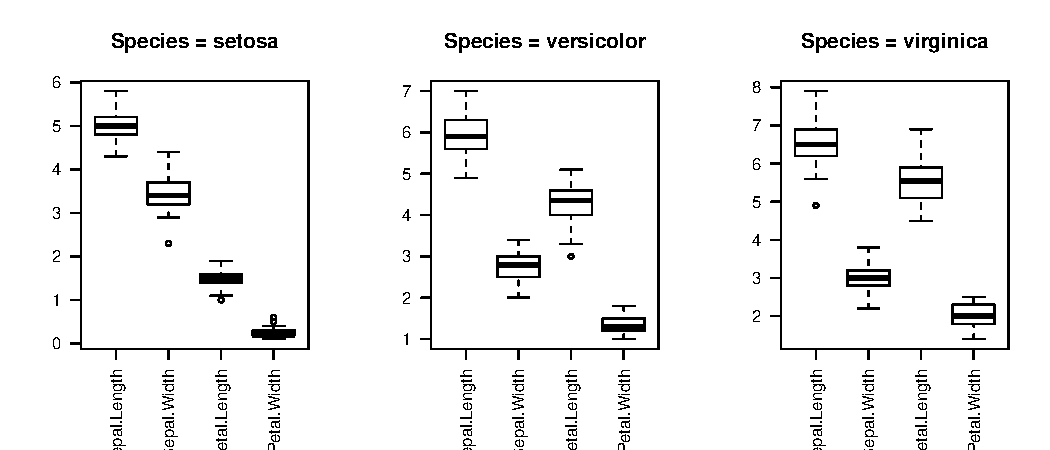
\includegraphics[width=\maxwidth]{figure/boxplots-1} 

}

\caption[Boxplots of the iris data for all three species]{Boxplots of the iris data for all three species}\label{fig:boxplots}
\end{figure}


\end{knitrout}
\blindtext[4]

For the boxplots, see \vref{fig:boxplots}.


% Conclusion:

\newpage
\section{Conclusion}
\label{sec:Conclusion}

\blindtext[4]

% References
\newpage
\setlength{\bibitemsep}{.45\baselineskip}
\bibliographystyle{apacite}
\interlinepenalty=10000  %prevent splited bibitems
\bibliography{References}

%%%%%%%%%%%%%%%%%%%%%%%%%%%%%%%%%%%%%%%%%%%%%%%%%%%%%%%%%%%%%%%%%%%%%%%%%%%%%%
%%%%%%%%%%%%%%%%%%%%%%%%%%%%%%%%%%% Appendix %%%%%%%%%%%%%%%%%%%%%%%%%%%%%%%%%
%%%%%%%%%%%%%%%%%%%%%%%%%%%%%%%%%%%%%%%%%%%%%%%%%%%%%%%%%%%%%%%%%%%%%%%%%%%%%%
\labelformat{section}{appendix~#1} % following sections are called appendix when refered to
\begin{appendices}
\newpage
\section{Data Declaration}
\blindtext



\newpage
\section{\R-Code}
\label{app:code}
\lstinputlisting[nolol=true,basicstyle=\scriptsize\tt,breaklines=true]{Code/functions.R}
\end{appendices}

%%%%%%%%%%%%%%%%%%%%%%%%%%%%%%%%%%%%%%%%%%%%%%%%%%%%%%%%%%%%%%%%%%%%%%%%%%%%%%
%%%%%%%%%%%%%%%%%%%%%%%%%%%%%%% Academic Honesty %%%%%%%%%%%%%%%%%%%%%%%%%%%%%
%%%%%%%%%%%%%%%%%%%%%%%%%%%%%%%%%%%%%%%%%%%%%%%%%%%%%%%%%%%%%%%%%%%%%%%%%%%%%%
\section*{Academic Honesty}
Ich erkl\"are hiermit,
\begin{itemize}
\item that I have written this work without any help from others and without the use of documents and aids other than those stated above,
\item that I have mentioned all the sources used and that I have cited them correctly according to established academic citation rules,
\item that the topic or parts of it are not already the object of any work or examination of another course unless this has been explicitly agreed on with the faculty member in advance,
\item that I will not pass on copies of this work to third parties or publish them without the University’s written consent if a direct connection can be established with the University of St.\,Gallen or its faculty members,
\item that I am aware that my work can be electronically checked for plagiarism and that I hereby grant the University of St.\,Gallen copyright in accordance with the Examination Regulations in so far as this is required for administrative action.
\end{itemize}
\vspace{1cm}
\hfill \theCity, \theDate
\\ 
\vspace{1.5cm}


\hfill \theAuthor
\thispagestyle{empty}

\end{document}
